% !TEX root = ../thesis-example.tex
%
\chapter{Introduction et contexte -- Géométrie digitale et projet digitalSnow}
\label{sec:introduction}

% \cleanchapterquote{We have seen that computer programming is an art, because it applies accumulated knowledge to the world, because it requires skill and ingenuity, and especially because it produces objects of beauty.}{Jean-Claude Vandamme}{Ma vie, mon œuvre.}

\setcounter{minitocdepth}{3}
\minitoc

\newpage

Depuis quelques années, nous vivons dans un monde entouré en permanence de
\colorize{données numériques}. Il ne passe pas un jour sans que nous ne soyons
bombardés de pixels, que ce soit sur les téléphones portables, les écrans
publicitaires animés, ou peut-être même actuellement si vous lisez ce document
sur un écran. Devant cette masse grandissantes de pixels, ou de voxels en
dimension 3, les besoins en traitement de ces données digitales sont de plus en
plus forts. Dans l'imagerie médicale par exemple, nous sommes capables de
récupérer de manière non-invasive un « amas de voxels » représentant un organe
d'un patient. Il existe une demande de plus en plus forte également pour la
sauvegarde du patrimoine culturel : les œuvres ont une durée de vie limitée par
le choix de leurs matériaux ou à cause d’événements extérieurs (guerres,
catastrophes naturelles), il devient alors préoccupant de les stocker
numériquement.

Le cadre de cette thèse, avec le \colorize{projet \digitalSnow}, est d'étudier
les métamorphoses de neige difficilement observable à l'œil nu grâce à leur
représentation digitale. Le projet \digitalSnow\footnote{ANR-11-BS02-009,
\url{http://liris.cnrs.fr/dsnow/}} est un projet de recherche financé par
l'Agence Nationale de le Recherche qui regroupe trois laboratoires spécialisé
dans des domaines différents : le laboratoire d'informatique
\textsc{\colorize{LIRIS}} de l'Université de Lyon, le laboratoire de
mathématiques \textsc{\colorize{LAMA}} de l'Université de Savoie Mont-Blanc, et
le Centre d'Études de la Neige \textsc{\colorize{CEN}} du Centre National de
Recherches Météorologiques. Lors d'une chute de neige, les cristaux de glace
s'accumulent sur le sol et forment un ensemble poreux d'air humide, de glace et
d'eau. Cette neige se transforme avec le temps, l'enjeu ici est de comprendre
comment évolue la micro-structure de la neige en fonction des conditions
extérieures et des phénomènes intrinsèques du matériau (tension de surface). Pour
ce faire, nous récupérons des images digitales de dimension 3 de
micro-échantillons de neige grâce à la micro-tomographie à rayons X et nous
cherchons à extraire des quantités topologiques et géométriques (comme la
courbure) afin de modéliser les propriétés physiques du matériau. Nous
préciserons le contexte applicatif dans le
\RefSection{sec:applications:digitalsnow}.

La \colorize{\DigitalGeometry} tente alors d'apporter des outils mathématiques
permettant d'exploiter pleinement ces données digitales. Ces outils proviennent
généralement de la géométrie euclidienne classique et sont adaptés pour des
données digitales (parties de $\Z^d$). Cependant, comme le dit Jean
\textsc{Françon} dans la préface de « Géométrie discrète et images numériques »
\cite{Coeurjolly2007Book}, la \DigitalGeometry n'est pas seulement l'étude
d'objets du monde réel dans l'espace digital, mais également l'étude de l'objet
digital lui-même. Ainsi, sous l'impulsion de Jean-Pierre \textsc{Reveillès} dès
1988, la géométrie arithmétique s'intéresse aux droites et cercles non plus
comme étant seulement le produit d’un algorithme de tracé mais définis
intrinsèquement dans la géométrie digitale, sans l’être par approximation du
continu.

La principale motivation est d'approcher au plus près la représentation digitale
de l'objet de sa version euclidienne. Ainsi nous nous intéressons aux questions
suivantes : comment récupérer des informations sur l'objet réel étudié lorsque
nous n'avons à notre disposition qu'une version approchée de celui-ci, sa
version discrétisée ? Pouvons-nous garantir la qualité des quantités estimées
sur les données digitales ? Après de rapides définitions des notions et outils
de base utilisés en géométrie digitale dans le \RefChapitre{sec:notions}, nous
proposons dans le \RefChapitre{sec:estimators} des estimateurs digitaux de
courbure en dimension 2 et 3 (courbure moyenne, courbures principales) avec des
preuves mathématiques garantissant la qualité des résultats (propriété de
convergence asymptotique uniforme). Nous adapterons ces estimateurs dans ce même
chapitre afin qu'ils ne nécessitent aucun paramètre. Ensuite, dans le
\RefChapitre{sec:applications}, nous dérivons ces estimateurs de courbure afin
de reconnaître les singularités d'un objet, en quelque sorte les arêtes de
l'objet sous-jacent à sa représentation digitale. Enfin, nous conclurons et nous
apporterons quelques perspectives résultant de ces travaux dans le
\RefChapitre{sec:conclusion}.
%
%
%
% En 2000, durant l'école d'hiver « Digital and Image Geometry » en Allemagne, une
% liste de « problèmes ouverts » en géométrie et en topologie digitale a été
% dressé \cite{Klette2000OpenProblems} afin d'orienter les recherches dans le
% domaines pour les années à venir. Depuis, dans cette liste beaucoup de réponses
% ont été apportées. Mais on y trouve par exemple le problème « Algorithmes
% d'estimation et preuves de convergence asymptotique ». Déjà à l'époque cela
% représentait un problème important pouvant faire avancer le domaine de la
% géométrie digitale.
%
% Cette transition s'est également opéré dans des domaines sensibles
%
%
% Les applications sont variés et en nombre. Dans l'imagerie
% médical, dans la sauvegarde du patrimoine culturel, dans la compréhension du
% monde vivant, il n'est pas rare de récolter et stocker des données digitales.
% Ces données brutes nécessitent des algorithmes pour les comprendre, les analyser
% et en extraire des informations pertinentes.
%
% \begin{figure}[t]
%     \begin{center}
%       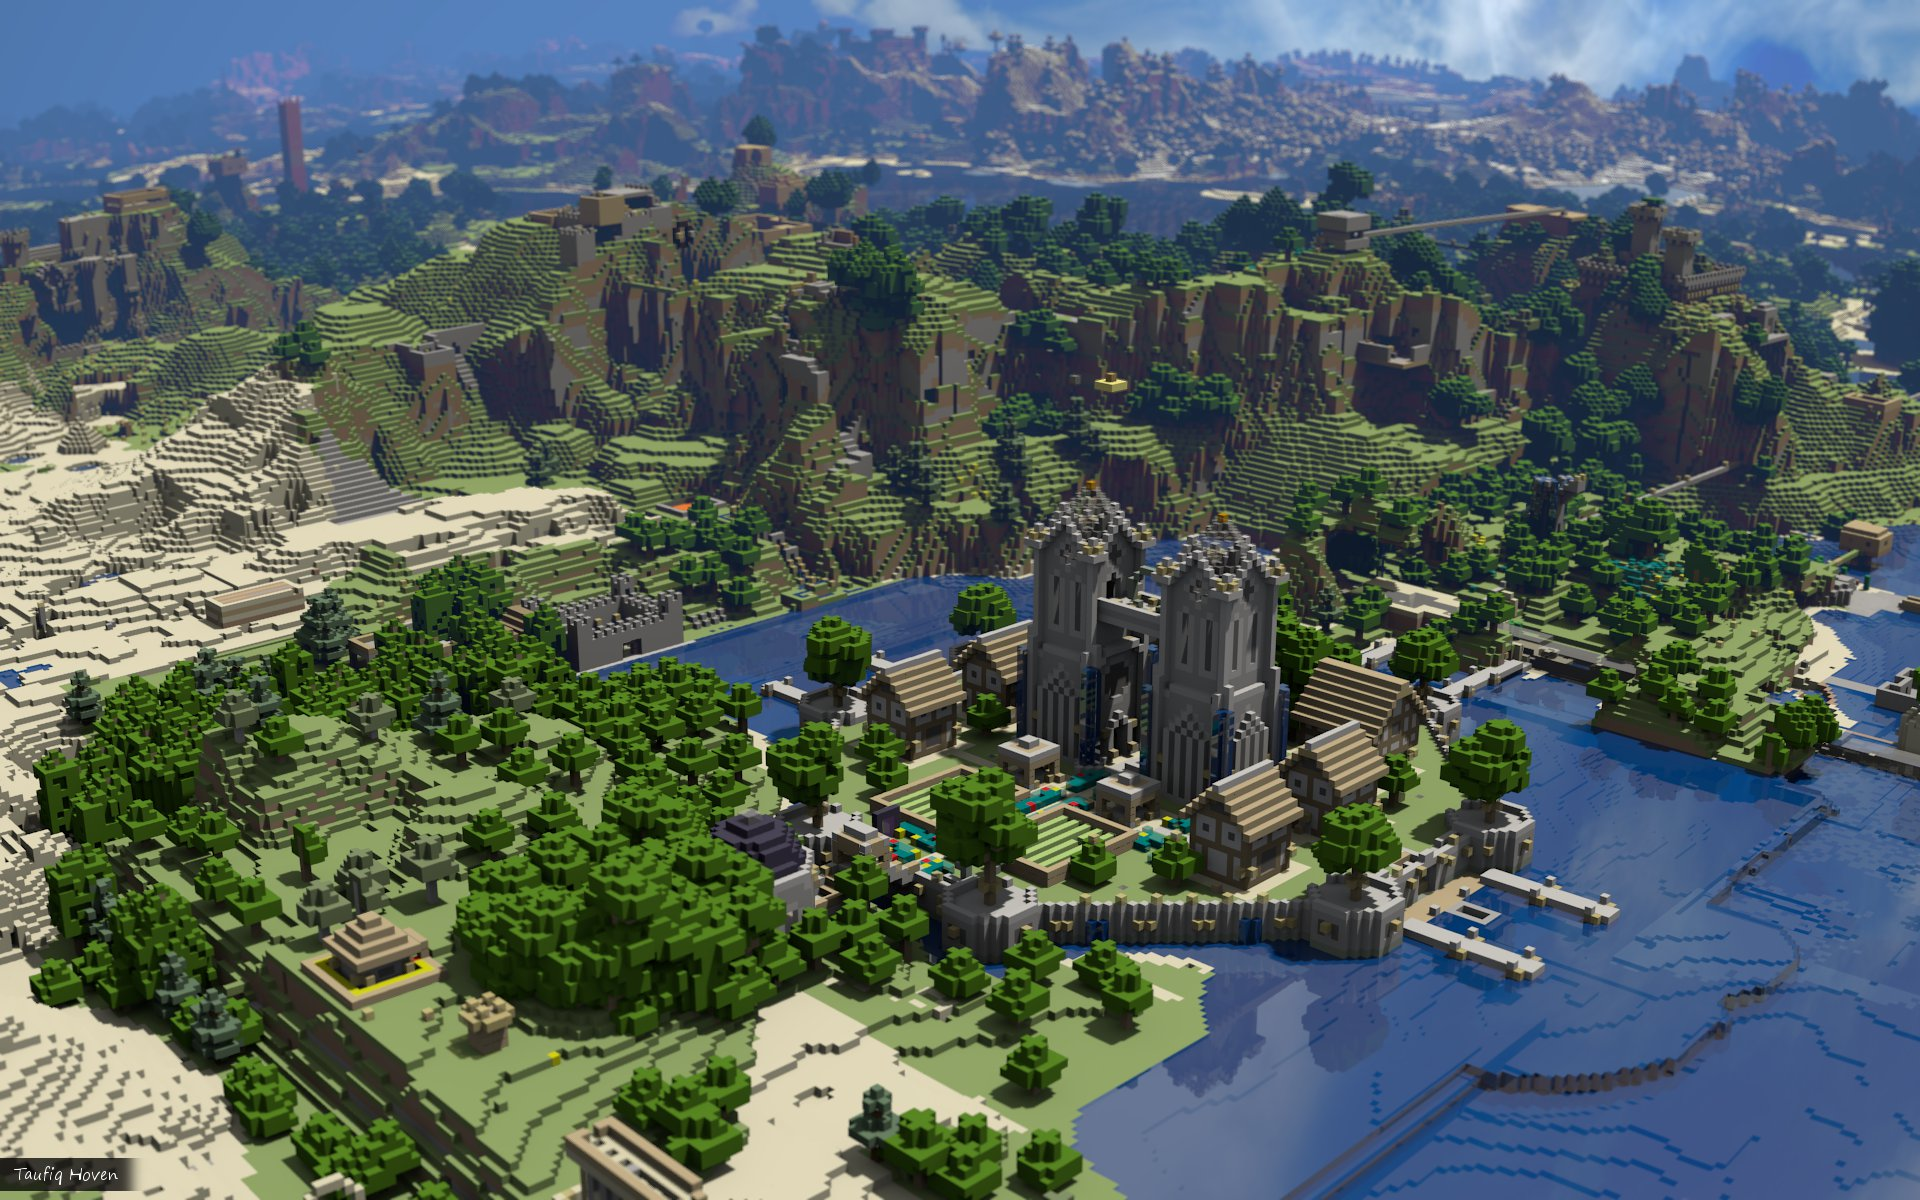
\includegraphics[width=14cm]{images/Introduction/minecraft-beautiful}
%     \end{center}
%     \caption{\textsc{Minecraft}, sorti en 2011 sur PC et plus tard sur consoles, représente un monde entièrement en voxels.}
%     \label{fig:minecraft}
% \end{figure}
%
% Un autre domaine en plein essort fait le pari des données digitales : le jeu
% vidéo. Certains moteurs de jeux ont fait le choix de basculer dans un
% environnement entièrement digital. L'exemple de jeu le plus connu est
% probablement \textsc{Minecraft}, sorti en 2011 sur PC : le joueur interagit avec
% un monde entièrement voxelique et permet de le modifier à sa guise (\RefFigure{fig:minecraft}). Un autre
% moteur comment à prendre sérieusement de l'ampleur : \textsc{Atomontage Engine}.
% Celui-ci propose de modéliser entièrement l'environnement en voxel et fait un
% post-traitement sur les données digitales afin d'avoir l'impression d'être sur
% des données continues.
%
% Ces données digitales sont l'objet de recherches intenses, même si le domaine
% reste relativement jeune.
